\documentclass[12pt,oneside,a4paper,english]{article}
\usepackage[T1]{fontenc}
\usepackage[latin2]{inputenc}
\usepackage[margin=2.25cm,headheight=26pt,includeheadfoot]{geometry}
\usepackage[english]{babel}
\usepackage{listings}
\usepackage{color}
\usepackage{titlesec}
\usepackage{titling}
\usepackage[framed, numbered]{matlab-prettifier}
\usepackage{changepage}
\usepackage{amsmath}
\usepackage{hyperref}
\usepackage{enumitem}
\usepackage{graphicx}
\usepackage{fancyhdr}
\usepackage{lastpage}
\usepackage{caption}
\usepackage{tocloft}
\usepackage{setspace}
\usepackage{multirow}
\usepackage{titling}
\usepackage{float}
\usepackage{comment}
\usepackage{booktabs}
\usepackage{indentfirst}
\usepackage{lscape}
\usepackage{booktabs,caption}
\usepackage[flushleft]{threeparttable}
\usepackage[english]{nomencl}
\usepackage{xcolor}
\usepackage{lipsum}
\usepackage{tcolorbox}

% --- set footer and header ---
\pagestyle{fancy}
\fancyhf{}

\setlength{\parindent}{2em}
\title{Title of the document} % to reference as \title, dont use \maketitle
\makeatletter\let\Title\@title\makeatother



\lstset{language=Matlab,
style=Matlab-editor,
basicstyle=\normalsize\mlttfamily,
numbers=left,
numberstyle={\scriptsize\color{black}},			% size of the numbers
numbersep=0.5cm											
}

\newlist{steps}{enumerate}{1}
\setlist[steps, 1]{leftmargin=1.5cm,label = Step \arabic*:}
\renewcommand{\headrulewidth}{1pt}
\renewcommand{\footrulewidth}{1pt}

%\lhead{\Title}
\rhead{\nouppercase{\rightmark}}
\lhead{\Title}
\rfoot{
\includegraphics[height=1.25cm]{root/logo.pdf}} % right header logo
\setlength\headheight{16pt}
\setlength{\footskip}{50pt}
\lhead{\Title} %rightH title
\cfoot{\thepage}

% --- End of page settings ---

% new theorem setting
\newtheorem{example}{Example}[section]
\newtheorem{discussion}{Discussion}[section]
% \newenvironment{solution}{\begin{example}[Solution]}{\end{example}}

\begin{document}
\pagenumbering{roman} 

\begin{titlepage}
\begin{center}
\vspace{2cm}
%\textsc{ Danmarks Tekniske Universitet}\\[1.5cm]

\includegraphics[width=0.4\textwidth]{root/dtu.png}~\\[1cm]
\vspace{2cm}

\vspace{2cm}

% Title
\hrule
\vspace{.5cm}
{ \huge \bfseries Title\\ of the report} % title of the report
\vspace{.5cm}

\hrule
\vspace{1.5cm}

\textsc{\textbf{Authors}}\\
\vspace{.5cm}
\centering

% add your name here
student - sxxxxxx\\
student - sxxxxxx\\

\vspace{4cm}

\centering \today % Dags dato
\end{center}
\end{titlepage}

\newpage
\doublespacing
%\addcontentsline{toc}{section}{Table of Contents}
\renewcommand{\baselinestretch}{1}\normalsize
\tableofcontents
\renewcommand{\baselinestretch}{1}\normalsize
%\singlespacing
\thispagestyle{fancy} % force page style

\newpage
\pagenumbering{arabic} 
\fancyfoot[C]{Page \thepage\ of \pageref{EndOfText}}

\section{Introduction} \label{ch1}
\subsection{What is an operating system?}
Special layer of software that provides application software access to hardware resources
\begin{itemize}
    \item Convenient \textbf{abstraction} of complex hardware devices
    \item Protected access to shared resources
    \item Security and authentication
    \item Communication amongst logical entities
\end{itemize}
\subsection{What Does an OS do?}
\paragraph{Provide abstractions to apps}File systems, Processes, threads, VM, containers, Naming system

\paragraph{Manage resources} Memory, CPU, storage,\dots

\paragraph{Achieves the above by implementing specific algos and techniques}Scheduling, Concurrency, Transactions, Security, \dots

\subsection{Illusionist}
Provide clean, easy-to-use \textbf{abstractions of physical resources}
\begin{itemize}
    \item Infinite memory, dedicated machine
    \item Higher level objects: files, users, messages
    \item Masking limitations, virtualization
\end{itemize}
\begin{figure}[H]
    \centering
    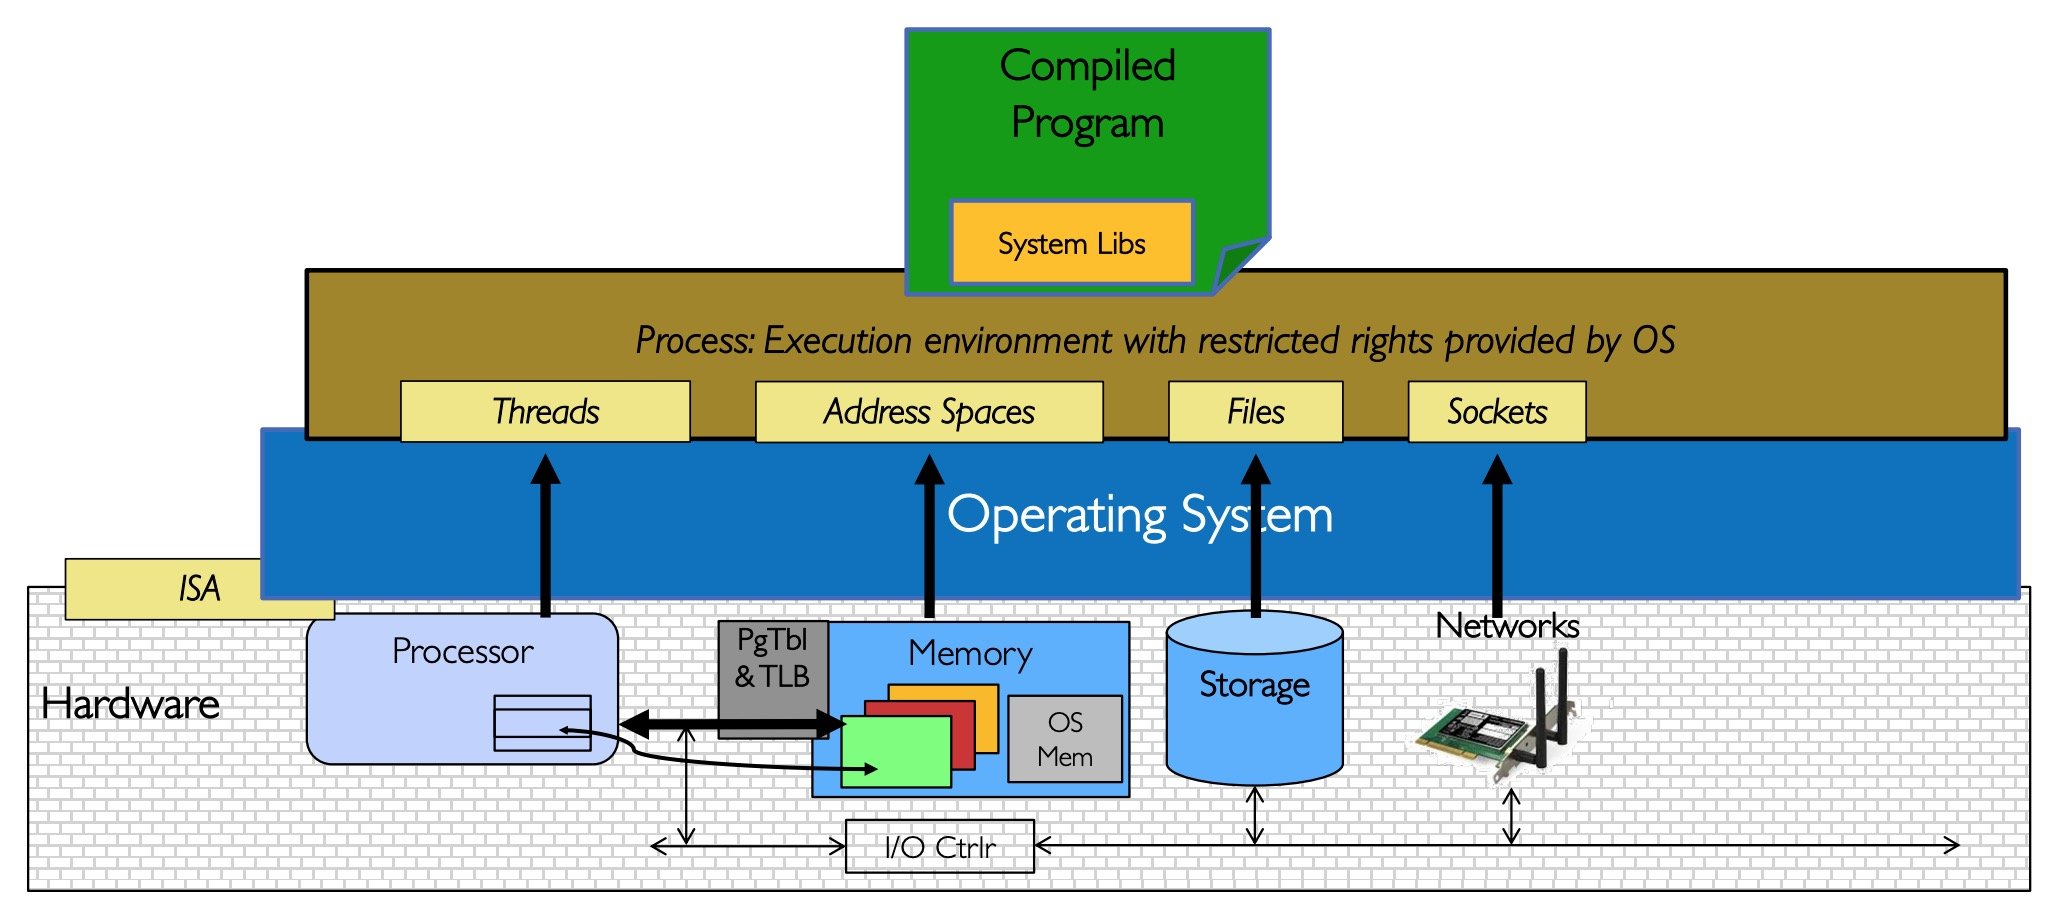
\includegraphics[width = 0.8\textwidth ]{figures/Virtualizing the Machine.jpg}
    \caption{Virtualizing the Machine}
    % \label{fig:batteryIncreas}
\end{figure}

\begin{figure}[H]
    \centering
    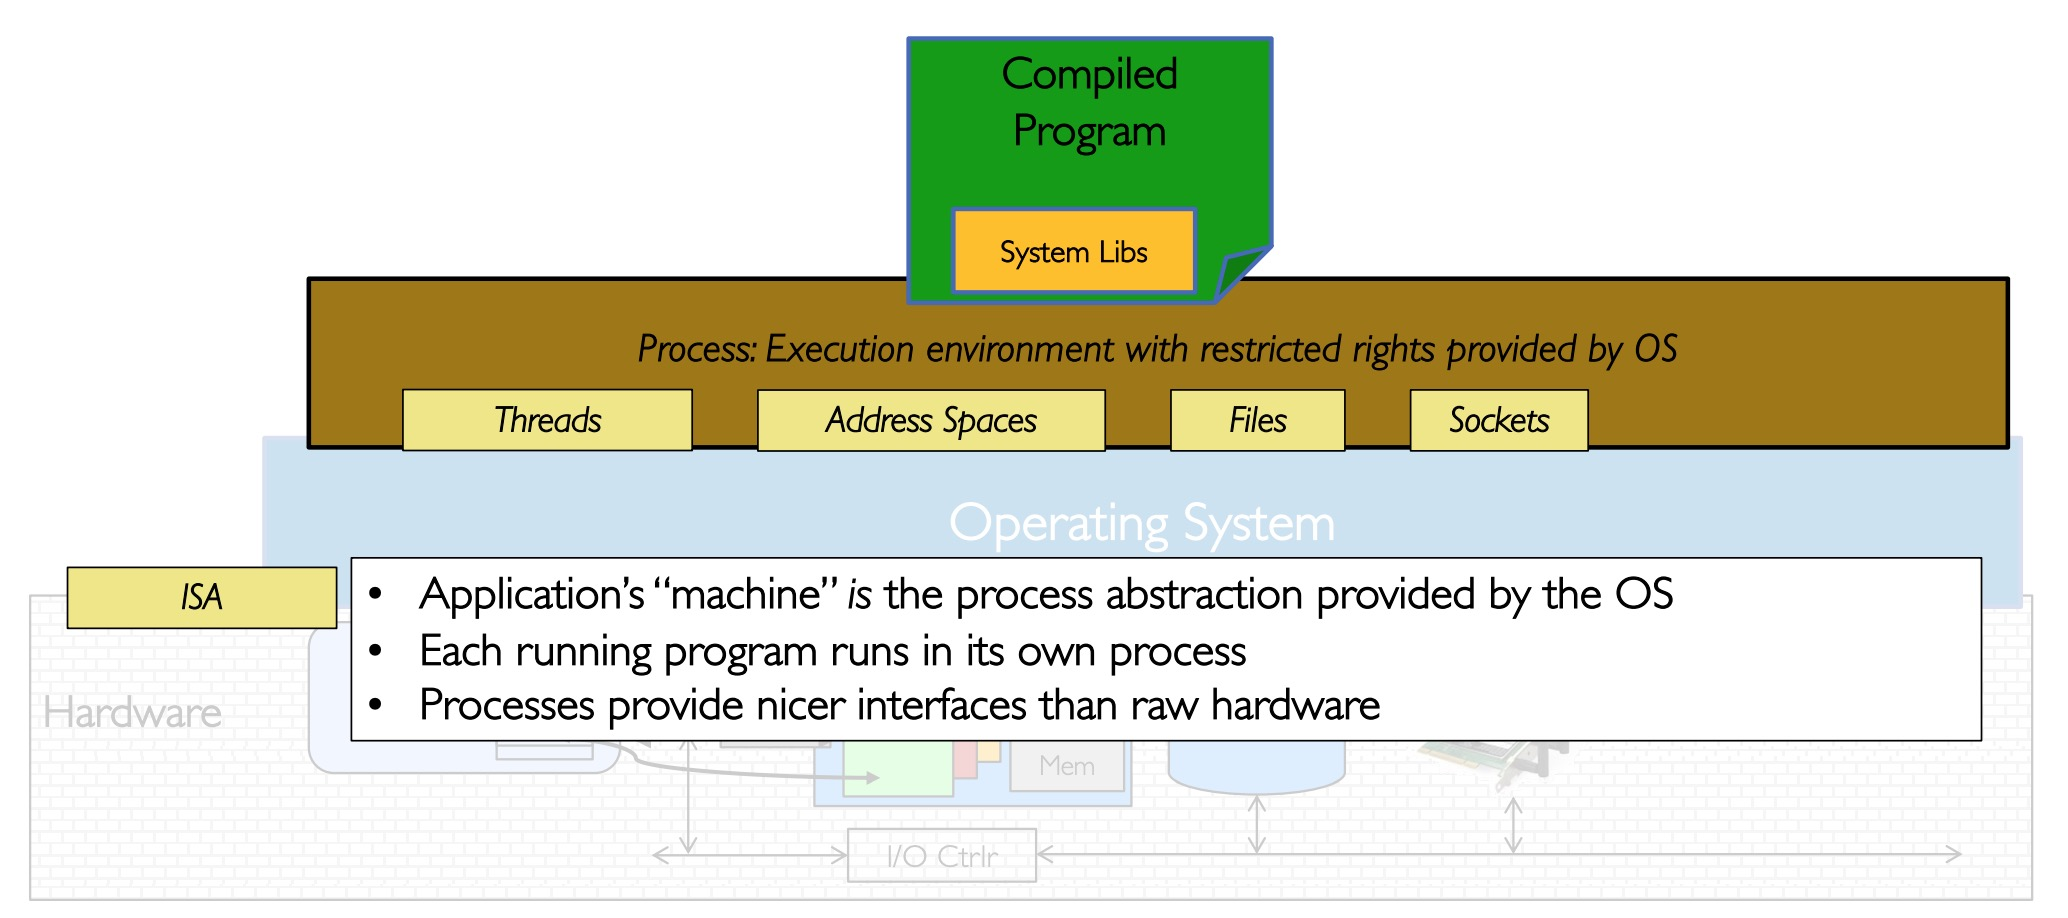
\includegraphics[width = 0.8\textwidth ]{figures/Compiled Program's View of the World.jpg}
    \caption{Compiled Program's View of the World}
    % \label{fig:batteryIncreas}
\end{figure}

\begin{figure}[H]
    \centering
    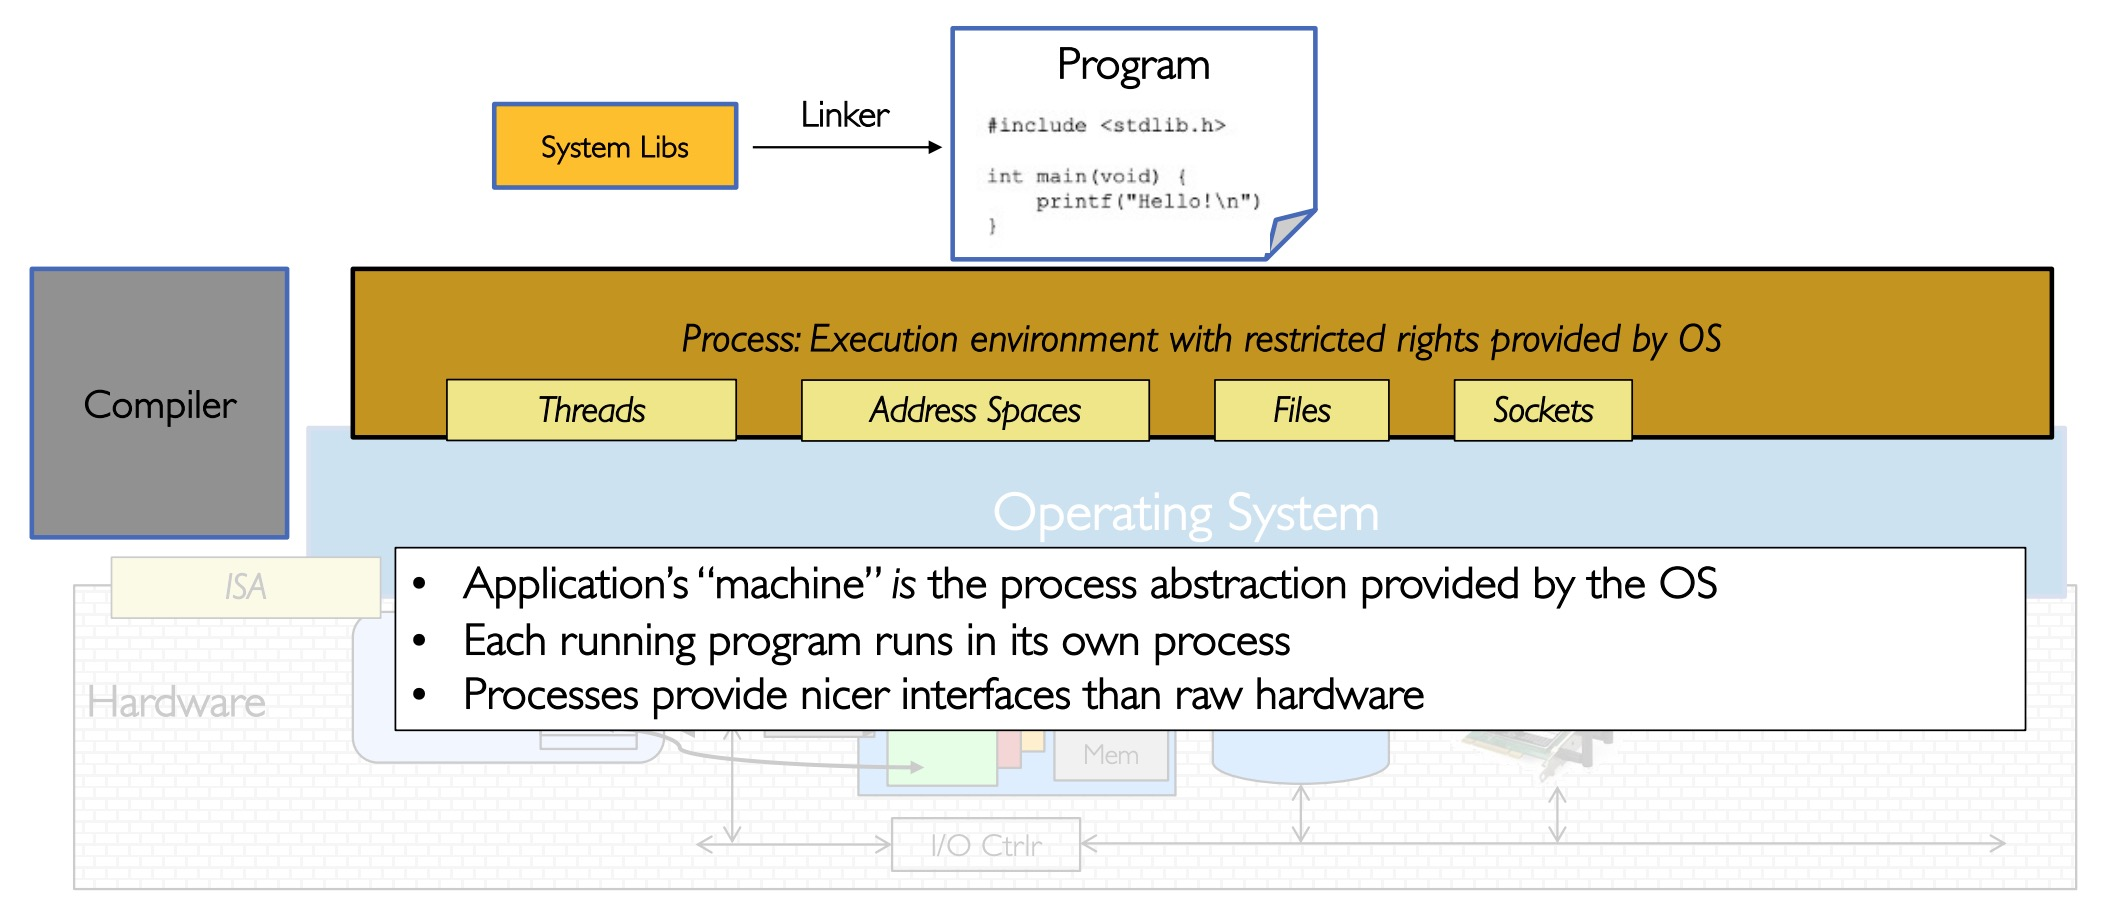
\includegraphics[width = 0.8\textwidth ]{figures/System Programmer's View of the World.jpg}
    \caption{System Programmer's View of the World}
    % \label{fig:batteryIncreas}
\end{figure}
\subsubsection{What's in a Process?}
\noindent A process consists of:
\begin{itemize}
    \item Address Space
    \item One or more threads of control executing in that address space
    \item Additional system state associated with it(Open files, Open sockets)
\end{itemize}
\begin{figure}[H]
    \centering
    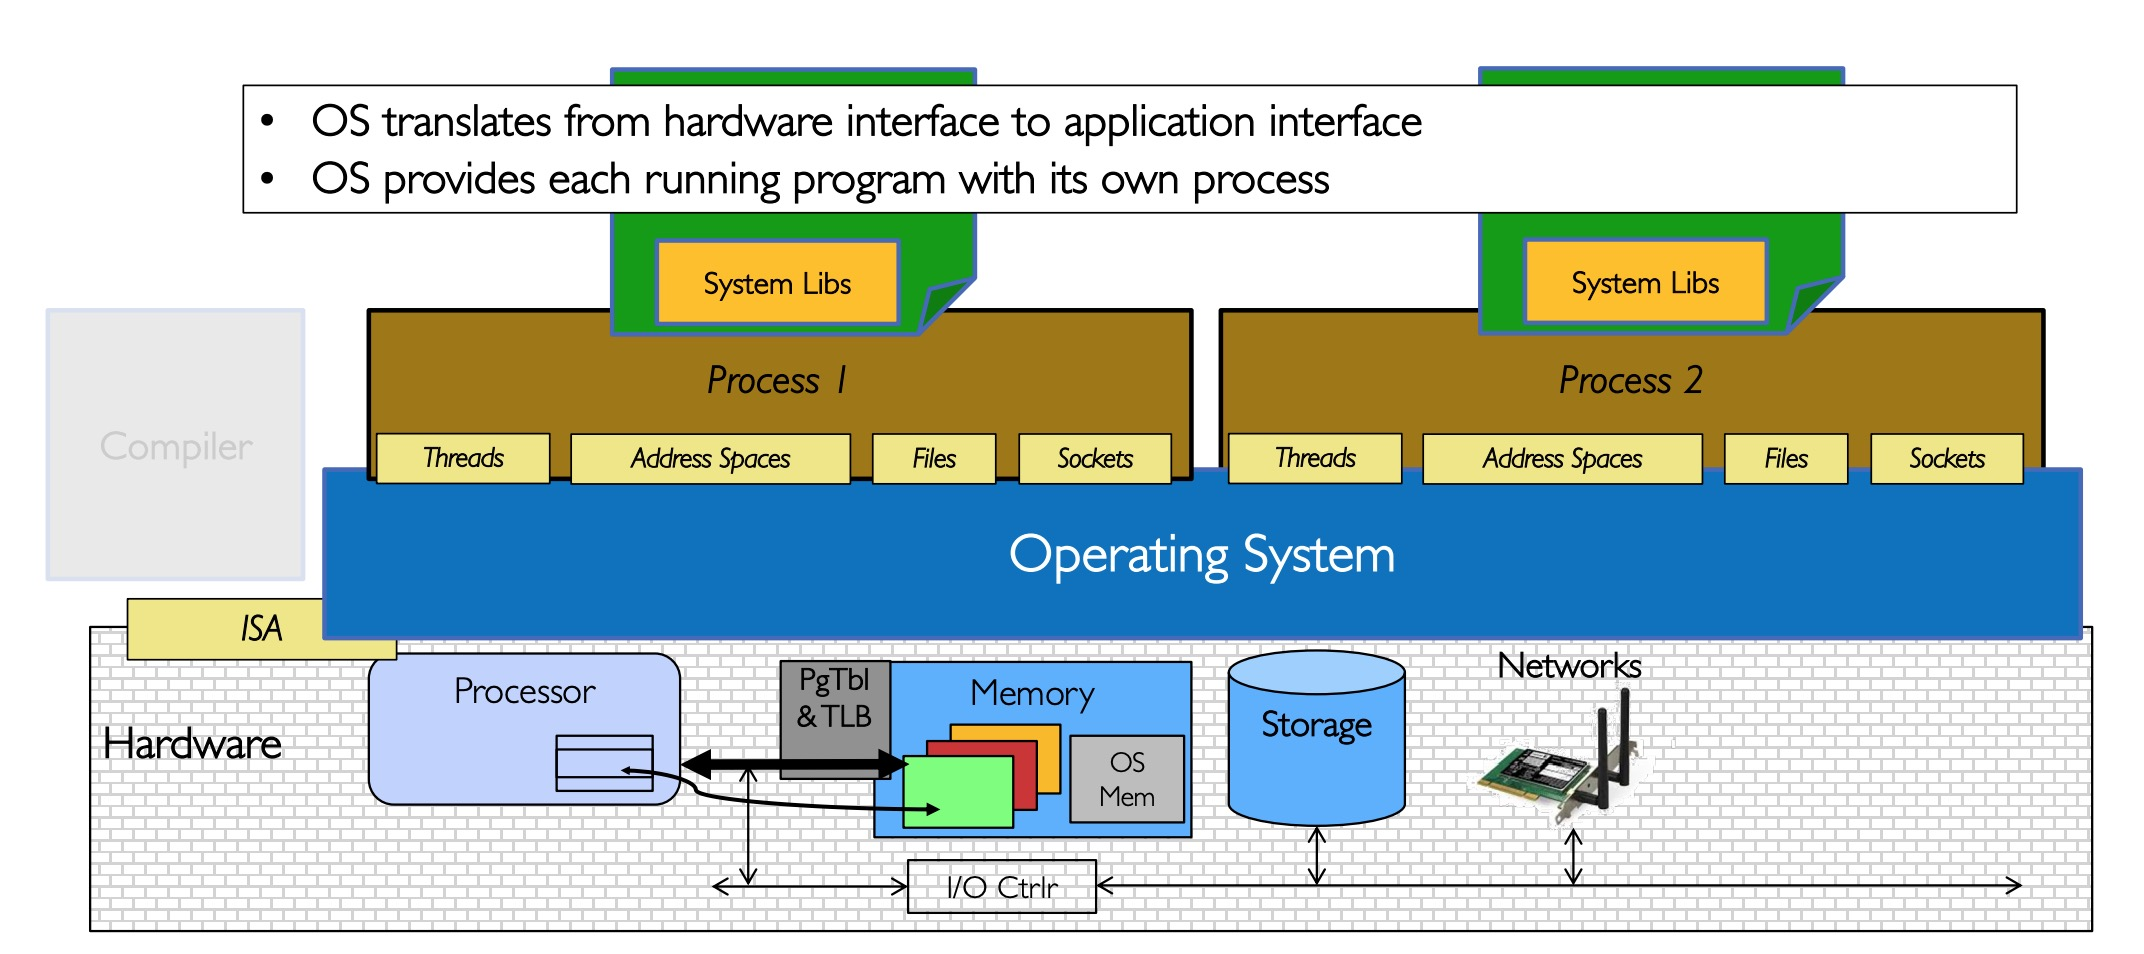
\includegraphics[width = 0.8\textwidth ]{figures/process_in_os_programmer_view.jpg}
    \caption{Process in System Programmer's View}
    % \label{fig:batteryIncreas}
\end{figure}

\subsection{Referee}
Manage \textbf{protection}, \textbf{isolation}, and \textbf{sharing of resources}
\begin{itemize}
    \item Resource allocation and communication
\end{itemize}
\begin{figure}[H]
    \centering
    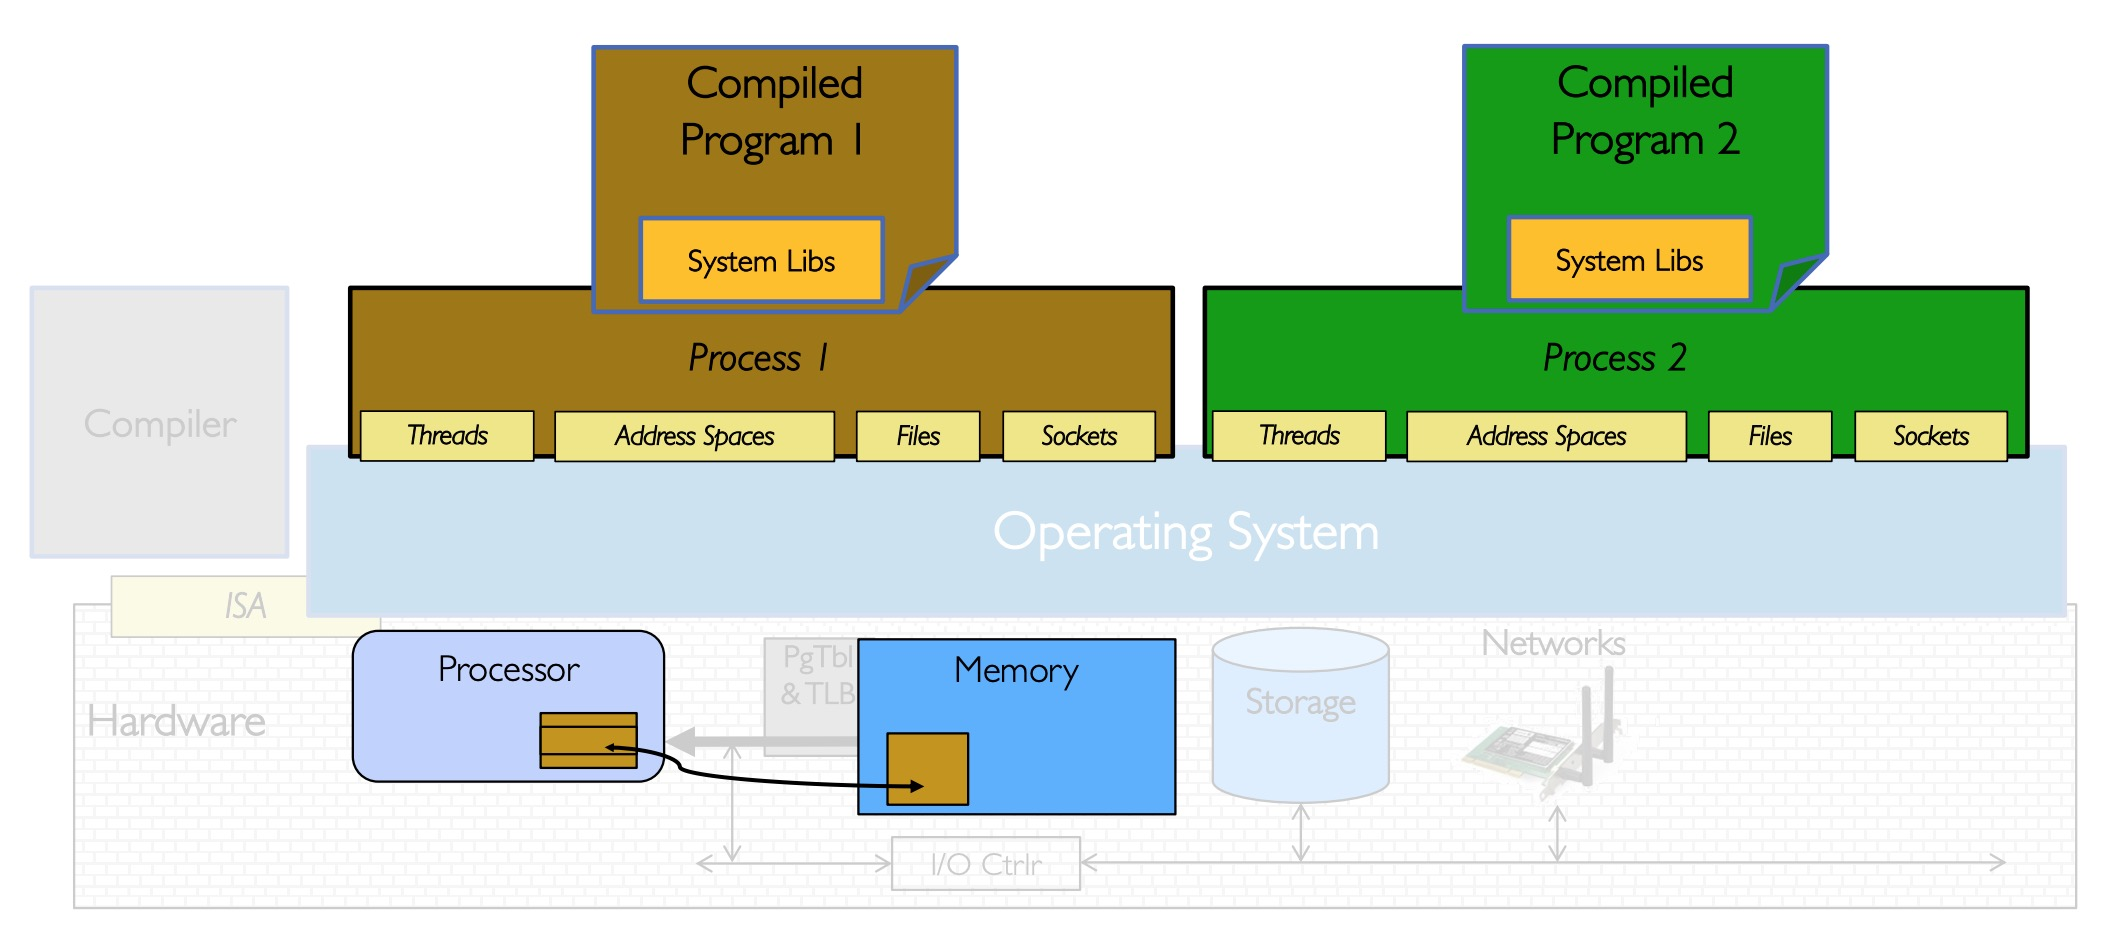
\includegraphics[width = 0.8\textwidth ]{figures/running_process.jpg}
    \caption{Running a Process}
    % \label{fig:batteryIncreas}
\end{figure}

\begin{figure}[H]
    \centering
    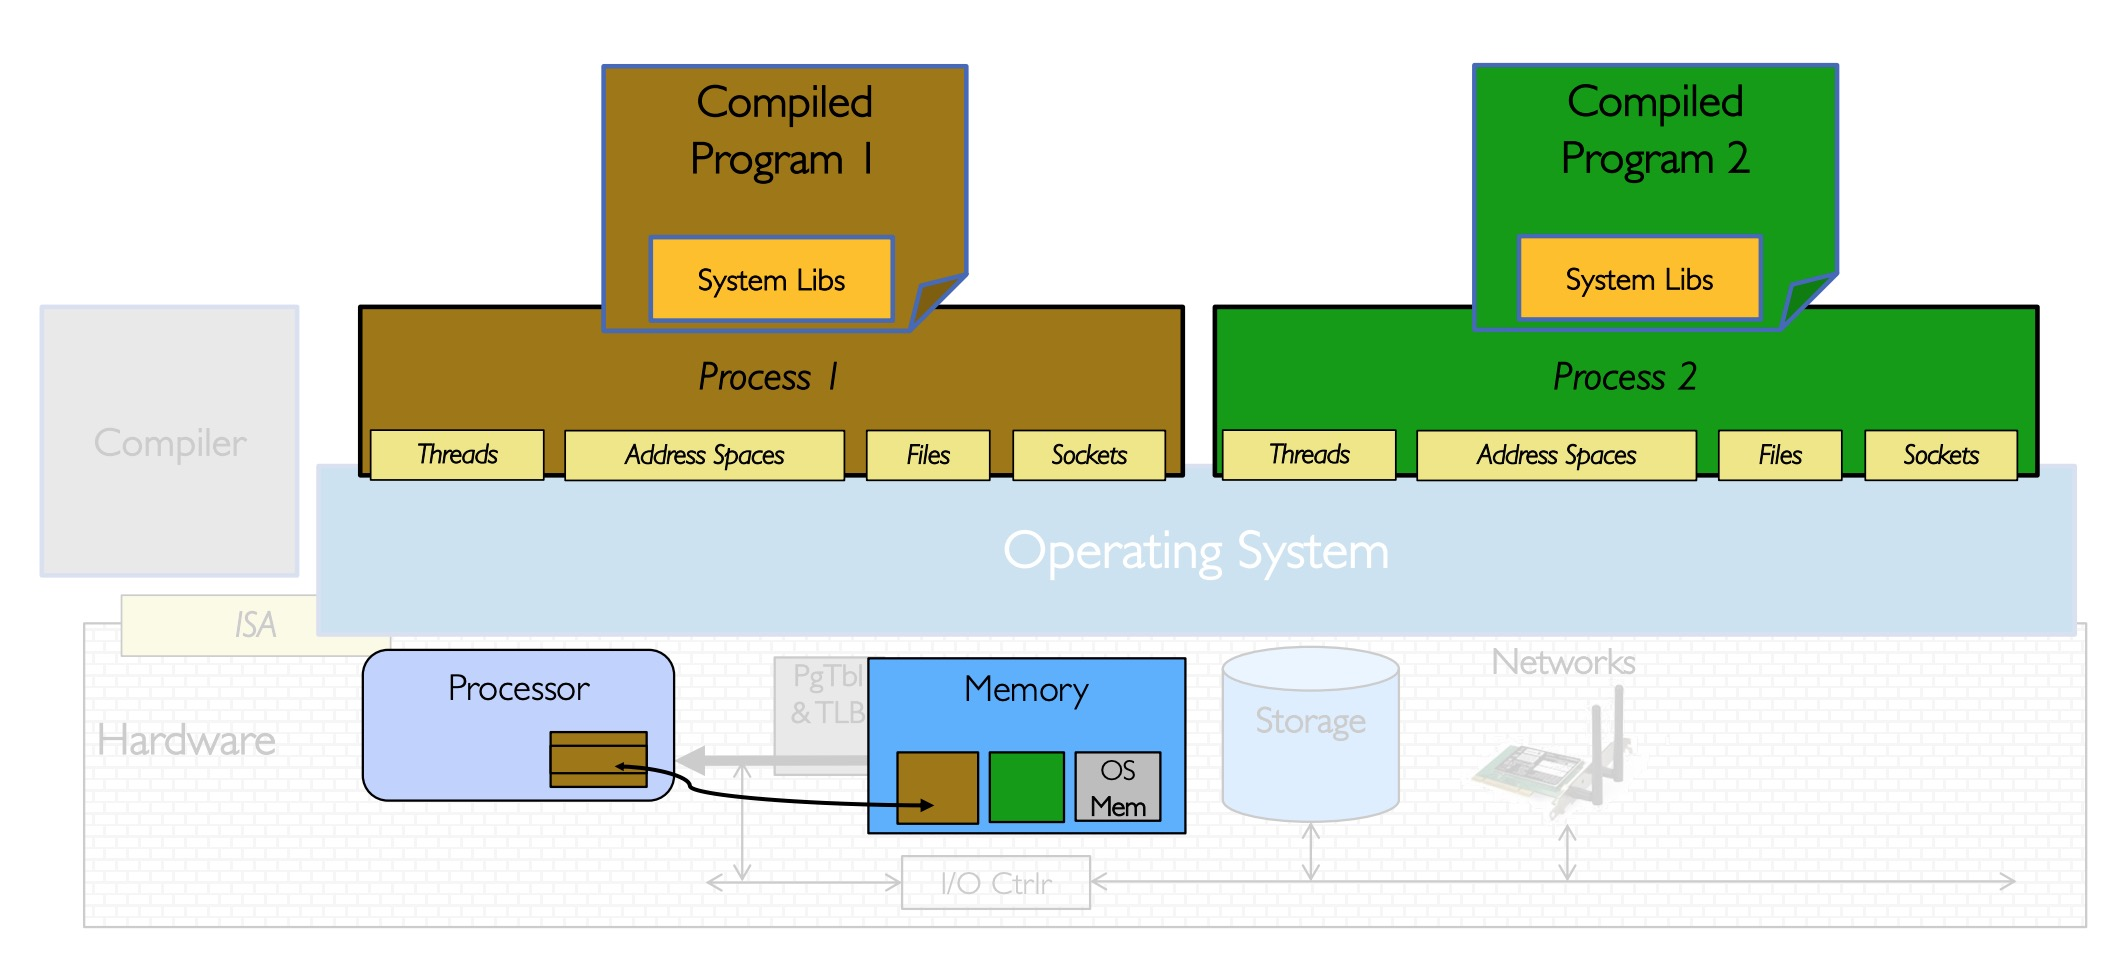
\includegraphics[width = 0.8\textwidth ]{figures/switching_process.jpg}
    \caption{Switching Process 1}
    % \label{fig:batteryIncreas}
\end{figure}
\subsubsection{Protection}
\begin{itemize}
    \item OS \textbf{isolates} processes from each other
    \item OS \textbf{isolates} itself from other processes
\end{itemize}
\begin{figure}[H]
    \centering
    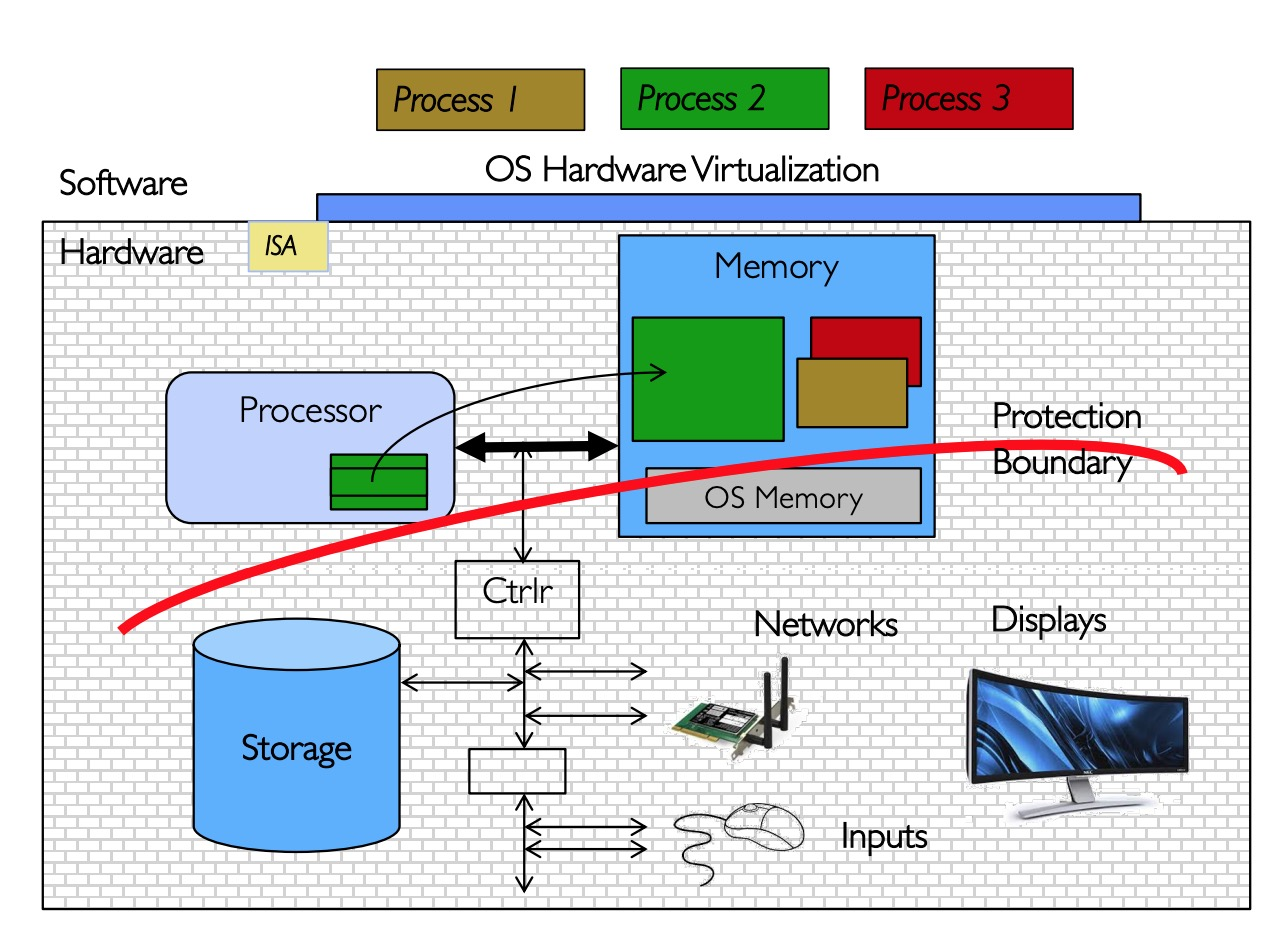
\includegraphics[width = 0.8\textwidth ]{figures/protection.jpg}
    \caption{Protection}
    % \label{fig:batteryIncreas}
\end{figure}

\subsection{Glue}
Common services
\begin{itemize}
    \item Storage, Window system, Networking
    \item Sharing, Authorization
    \item Look and feel
\end{itemize}
\subsubsection{I/O}
OS provides common services in the form of I/O

\begin{figure}[H]
    \centering
    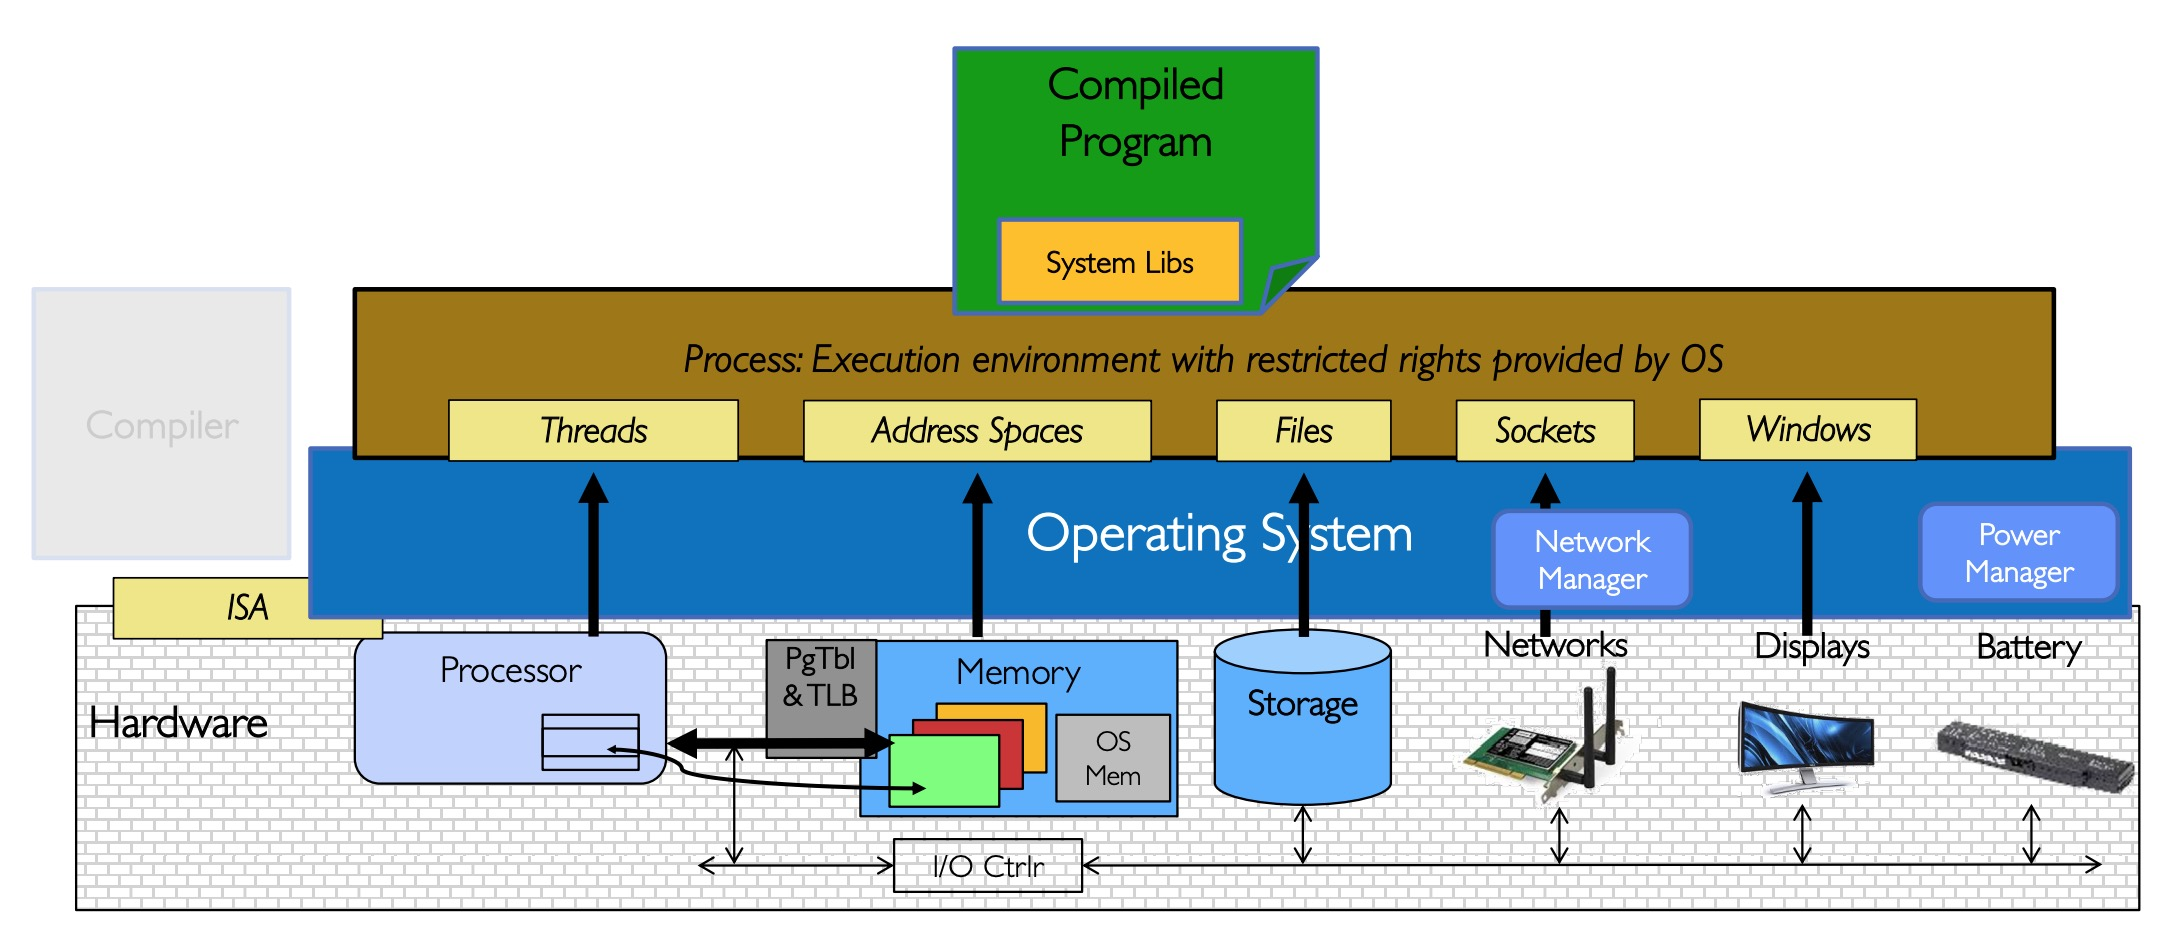
\includegraphics[width = 0.8\textwidth ]{figures/background_management.jpg}
    \caption{Background Management}
    % \label{fig:batteryIncreas}
\end{figure}

\begin{tcolorbox}
\begin{discussion}
How do we tame complexity?
\end{discussion}
\paragraph{Virtual Machine Abstraction} For software engineering Problem, system will turn hardware/software quirks to what programmers want/need
\begin{figure}[H]
    \centering
    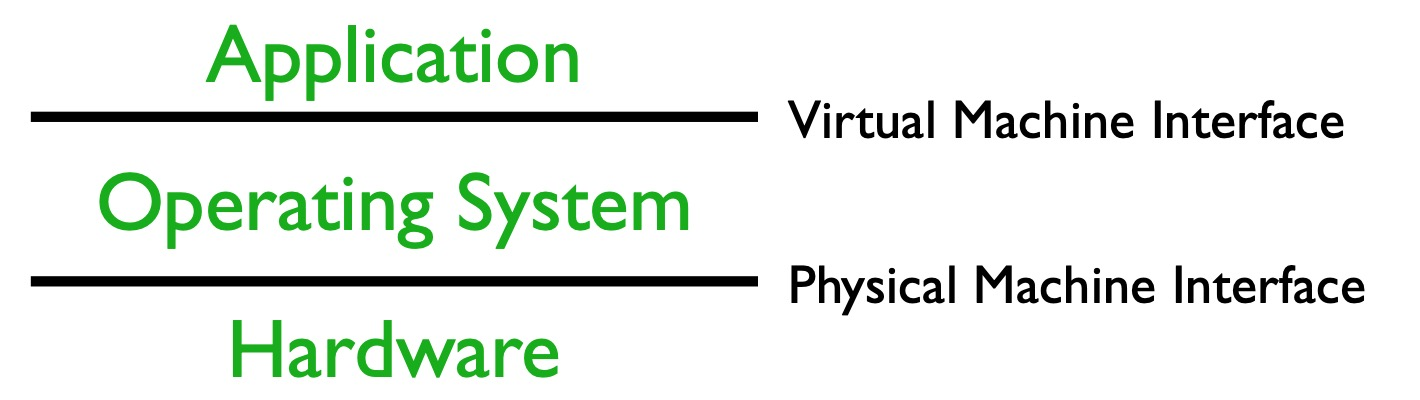
\includegraphics[width = 0.6\textwidth ]{figures/vma.jpg}
    \caption{Virtual Machine Abstraction}
    % \label{fig:batteryIncreas}
\end{figure}
\end{tcolorbox}

\subsection{Virtual Machine}
Two types of Virtual Machine:
\begin{itemize}
    \item \textbf{Process VM:} supports the execution of a single program; this functionality typically provided by OS
\item \textbf{System VM:} supports the execution of an entire OS and its applications (e.g.,
VMWare Fusion, Virtual box, Parallels Desktop, Xen)
\end{itemize}

\subsubsection{Process VMs}
\textbf{Programming simplicity}
\begin{itemize}
    \item Each process thinks it has \textbf{all} memory/CPU time
    \item Each process thinks it owns \textbf{all} devices
    \item Different devices appear to have \textbf{same} high level interface
    \item Device interfaces more powerful than raw hardware
\end{itemize}
\textbf{Fault Isolation}
\begin{itemize}
    \item Processes \textbf{unable} to\textbf{ directly impact other processes}
    \item Bugs \textbf{cannot} crash whole machine
\end{itemize}
\textbf{Protection and Portability}
\begin{itemize}
    \item Java interface safe and stable across many platforms
\end{itemize}

\subsubsection{System Virtual Machines: Layers of OSs}
Useful for OS development
\begin{itemize}
    \item When OS crashes, restricted to one VM
    \item Can aid testing programs on other OSs
\end{itemize}
\begin{figure}[H]
    \centering
    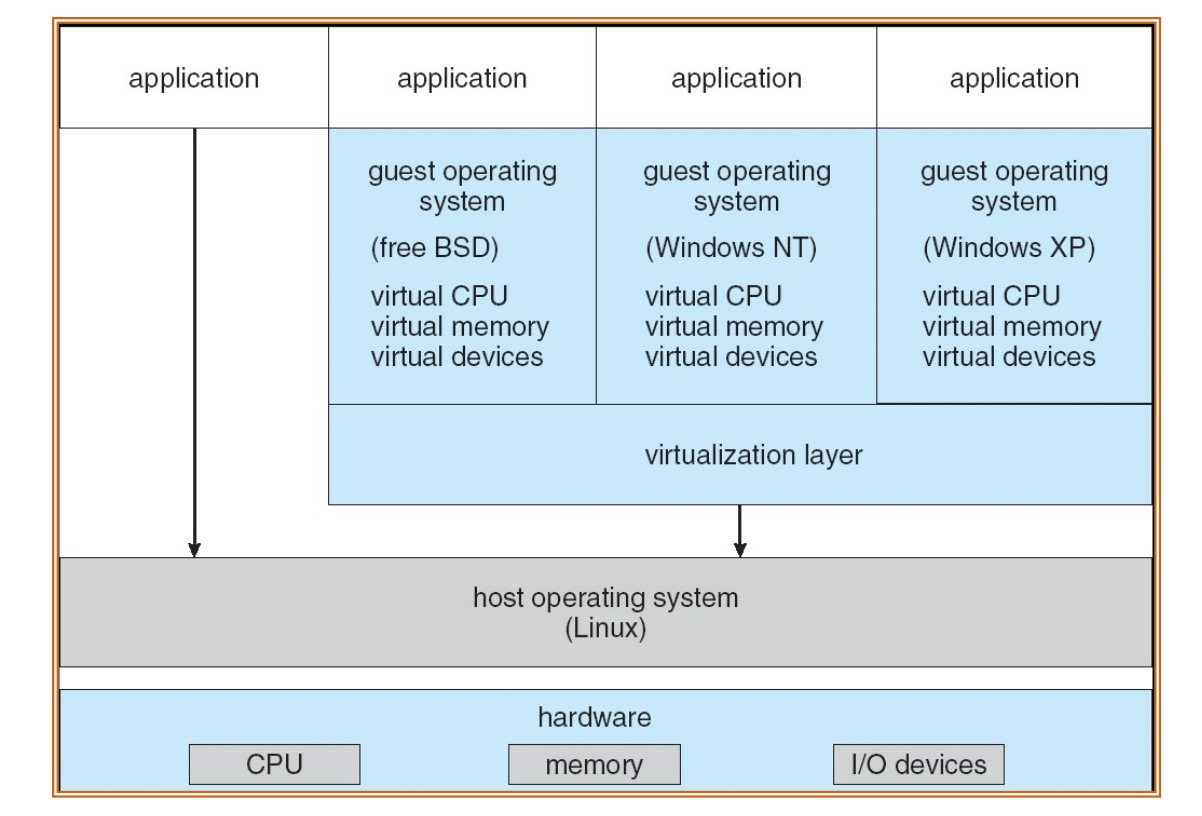
\includegraphics[width = 0.6\textwidth ]{figures/vm.jpg}
    \caption{Virtual Machine}
    % \label{fig:batteryIncreas}
\end{figure}



% \begin{figure}[H]
%     \centering
%     
\includegraphics[width = 0.8\textwidth ]{figures/tex.png}
%     \caption{Increase of battery capacity. }
%     \label{fig:batteryIncreas}
% \end{figure}


% In \autoref{tab:table1}

% \begin{table}[H]
%     \centering
%     \caption{That is a table.}
%     \begin{tabular}{|c|c|c|}
%     \centering
%     \textbf{Lorem} & \textbf{Ipsum} & \textbf{Lorem [\$]} \\ \hline \hline
% 1   & lipsum    & lorem     \\ \hline   
% 2   & lipsum    & lorem   \\ \hline
% 3   & lipsum    & lorem  
%     \end{tabular}
%     \label{tab:table1}
% \end{table}



\newpage
\section{Four Fundamental OS Concepts} \label{ch2}
\noindent\textbf{Thread}
\begin{itemize}
    \item single unique execution context: fully describes program state
    \item Program Counter, Registers, Execution Flags, Stack
\end{itemize}
\textbf{Address space (with translation)}
\begin{itemize}
    \item Programs execute in an address space that is distinct from the memory
space of the physical machine
\end{itemize}
\textbf{Process}
\begin{itemize}
    \item An instance of an executing program is a process consisting of an address space and one or more threads of control
\end{itemize}
\textbf{Dual mode operation / Protection}
\begin{itemize}
    \item Only the ``system'' has the ability to access certain resources
    \item The OS and the hardware are protected from user programs and user programs are isolated from one another by controlling the translation from program virtual addresses to machine physical addresses
\end{itemize}
\begin{discussion}
How do we run programs?
\end{discussion}
\begin{figure}[H]
    \centering
    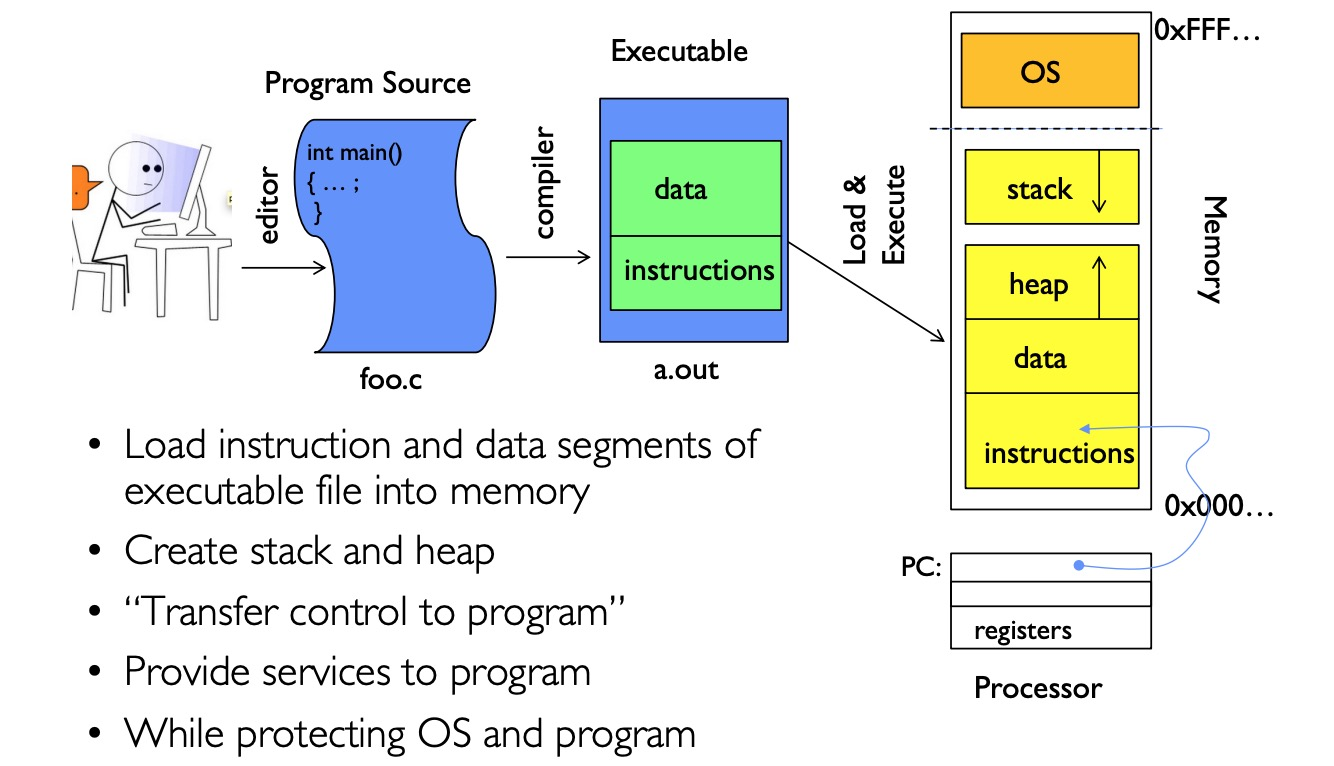
\includegraphics[width = 0.6\textwidth ]{figures/run_program.jpg}
    \caption{Run a Program}
    % \label{fig:batteryIncreas}
\end{figure}

\begin{discussion}
What happens during program execution?
\end{discussion}
\begin{figure}[H]
    \centering
    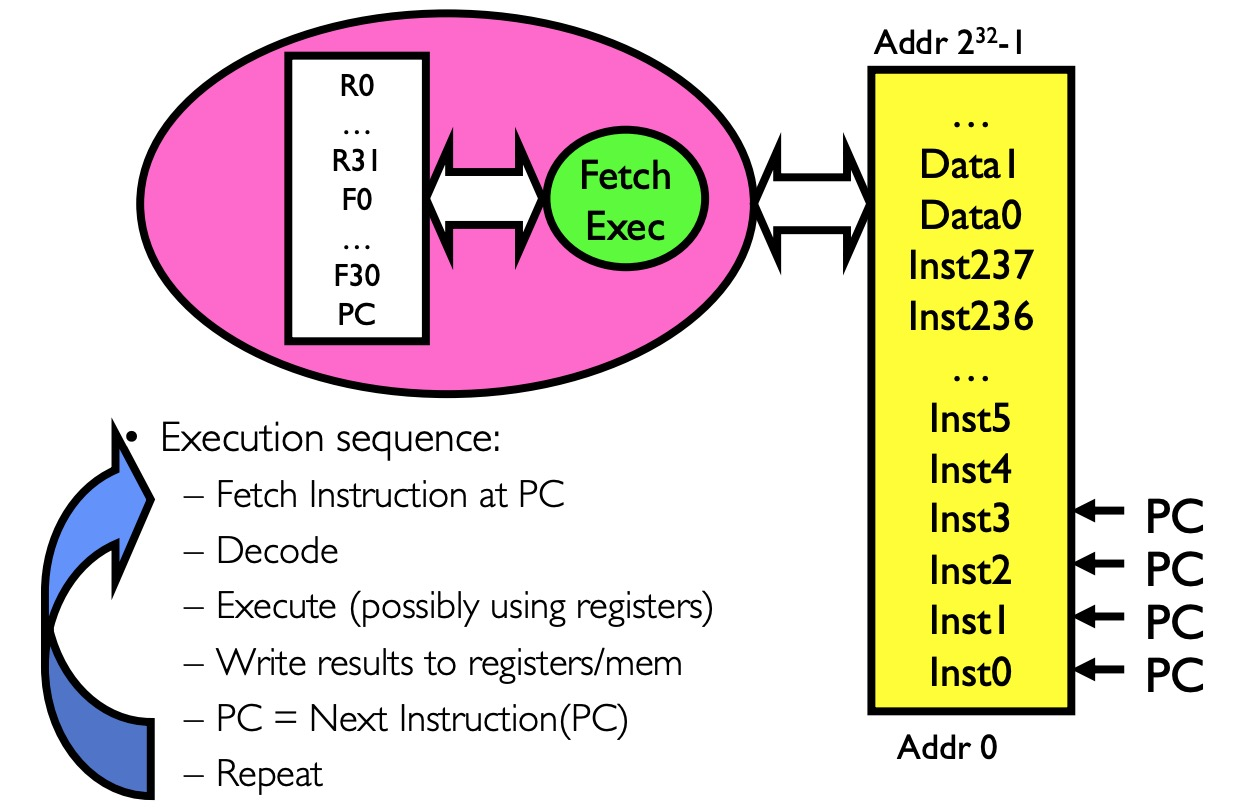
\includegraphics[width = 0.6\textwidth ]{figures/What_happens_during_program_execution?.jpg}
    \caption{What happens during program execution?}
    % \label{fig:batteryIncreas}
\end{figure}
\subsection{First OS Concept: Thread of Control}
\textbf{Thread}: Single unique execution context: \textbf{Program Counter, Registers, Execution Flags, Stack}
\begin{itemize}
    \item \textbf{Certain registers} hold the context of thread
    \item A thread is executing on a processor when it is resident in the processor register
    \item PC register holds the address of executing instruction in the thread
    \item Registers hold the root state of the thread
    \begin{itemize}
        \item The rest is ``in memory''
    \end{itemize}
\end{itemize}


\subsection{Second OS Concept: Program's Address Space}

\subsection{Third OS Concept: Process}
\begin{figure}[H]
    \centering
    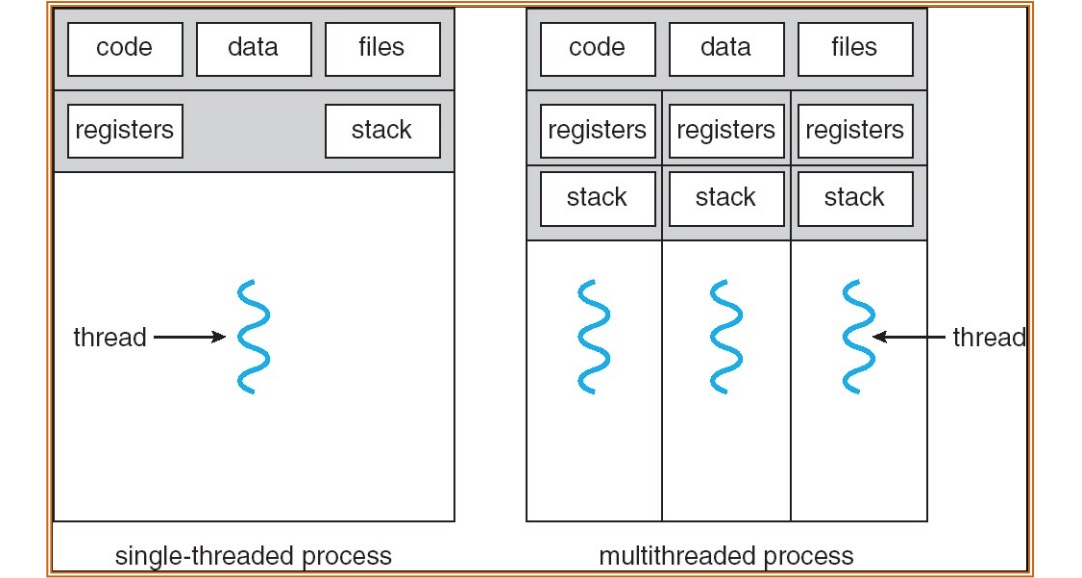
\includegraphics[width = 0.6\textwidth ]{figures/process.jpg}
    \caption{Single and Multithreaded Processes}
    % \label{fig:batteryIncreas}
\end{figure}


\subsection{Fourth OS Concept: Dual Mode Operation}
\begin{figure}[H]
    \centering
    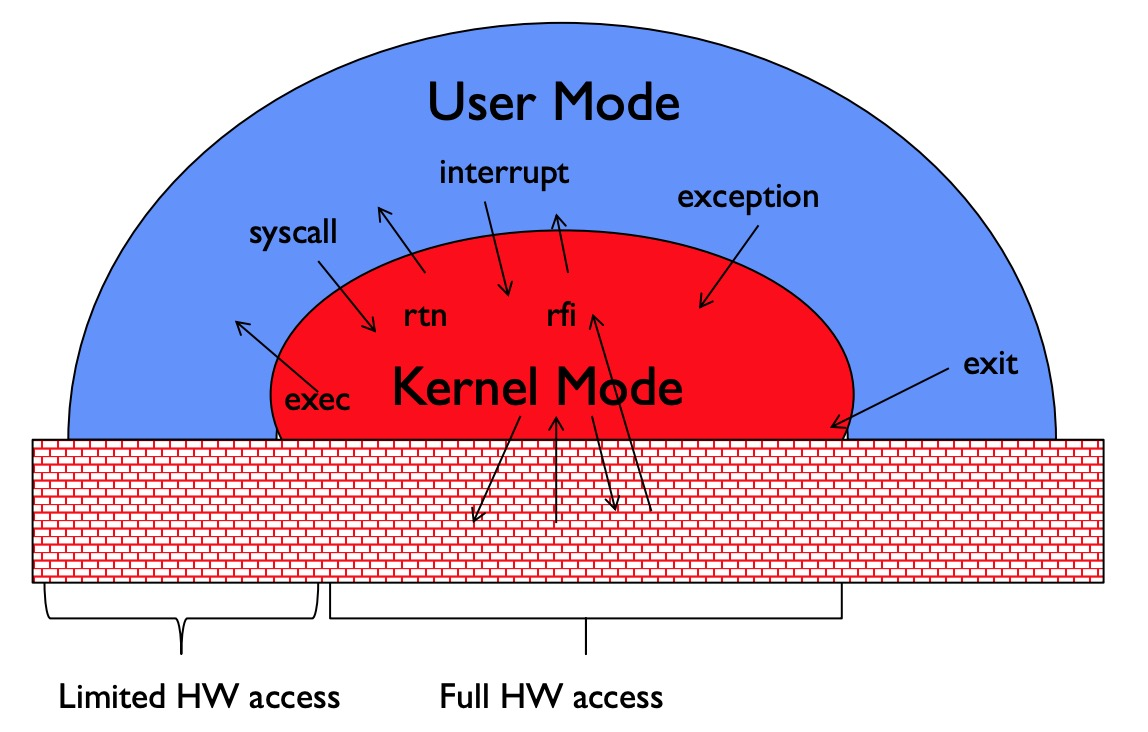
\includegraphics[width = 0.6\textwidth ]{figures/dual_mode.jpg}
    \caption{User/Kernel (Privileged) Mode}
    % \label{fig:batteryIncreas}
\end{figure}
\subsubsection{3 types of Mode Transfer}
\begin{itemize}
    \item \textbf{Syscall}
    \begin{itemize}
        \item Process requests a system service, e.g., exit
        \item Like a function call, but ``outside'' the process
        \item Does not have the address of the system function to call
        \item Like a Remote Procedure Call (RPC)
        \item Marshall the syscall id and args in registers and exec syscall
    \end{itemize}
    \item \textbf{Interrupt}
    \begin{itemize}
        \item External asynchronous event triggers context switch
        \item e. g., Timer, I/O device
        \item \textbf{Independent} of user process
    \end{itemize}
    \item \textbf{Trap or Exception}
    \begin{itemize}
        \item Internal synchronous event in process triggers context switch
        \item e.g., Protection violation (segmentation fault), Divide by zero, \dots
    \end{itemize}
\end{itemize}

\newpage
\section{Abstraction} \label{ch3}
\subsection{Thread}
\subsubsection{Protection}
\textbf{Simple Protection: Base and Bound (B\&B)}
\begin{figure}[H]
    \centering
    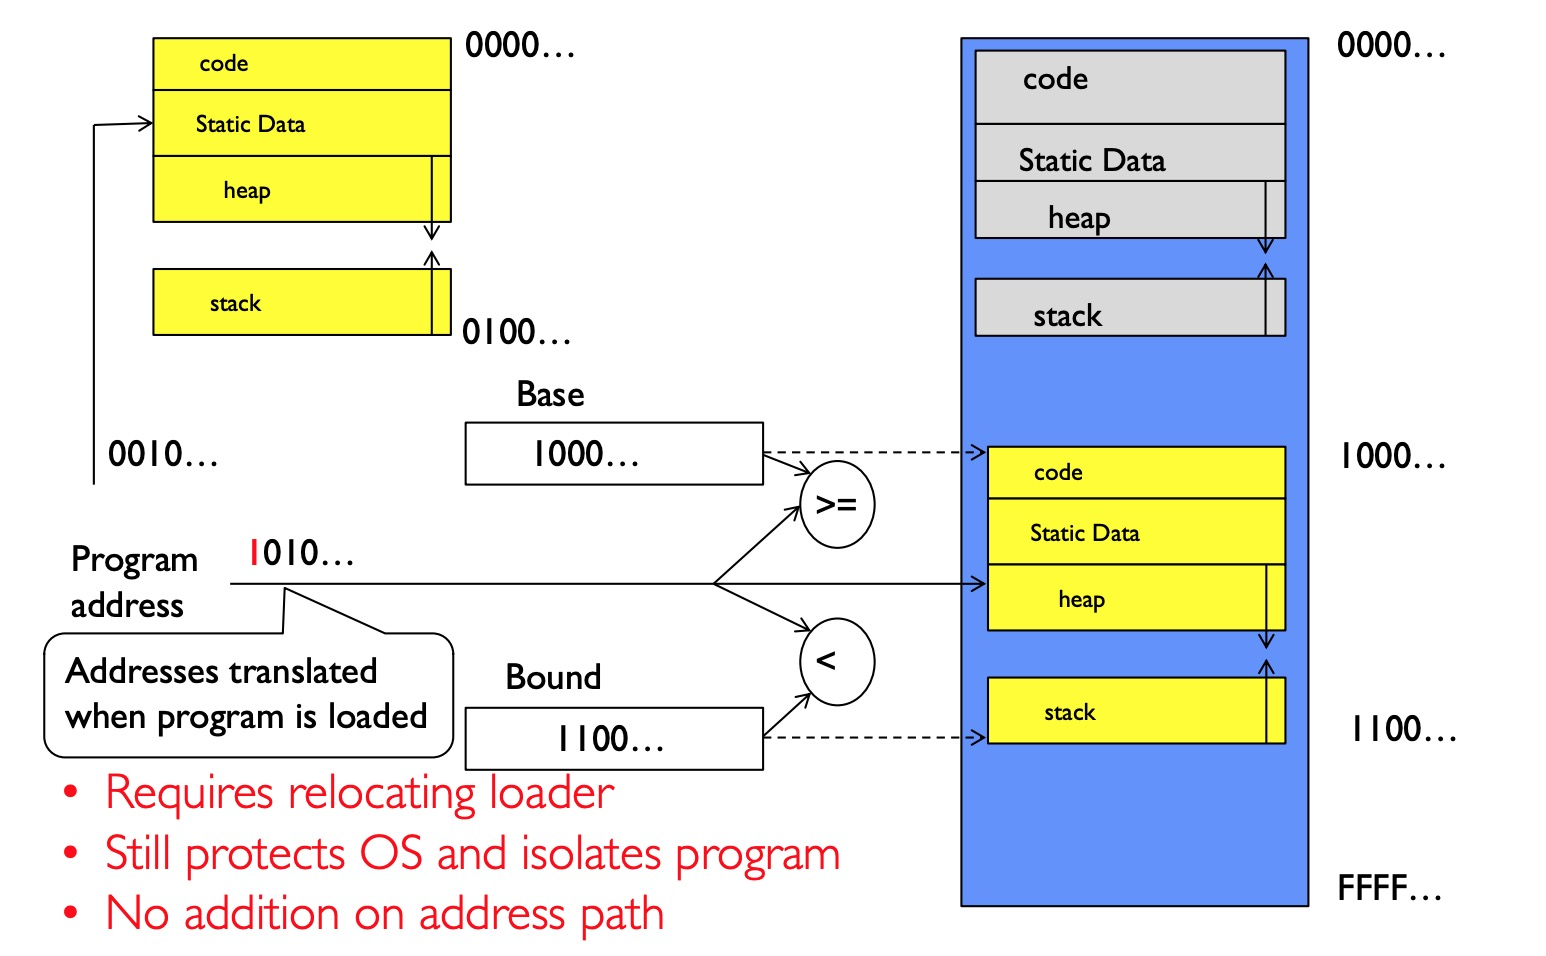
\includegraphics[width = 0.6\textwidth ]{figures/base_bound.jpg}
    \caption{Base and Bound}
    % \label{fig:batteryIncreas}
\end{figure}

\textbf{Another idea: Address Space Translation}
Program operates in an address space that is \textbf{distinct from the physical memory space of the machine}
\begin{figure}[H]
    \centering
    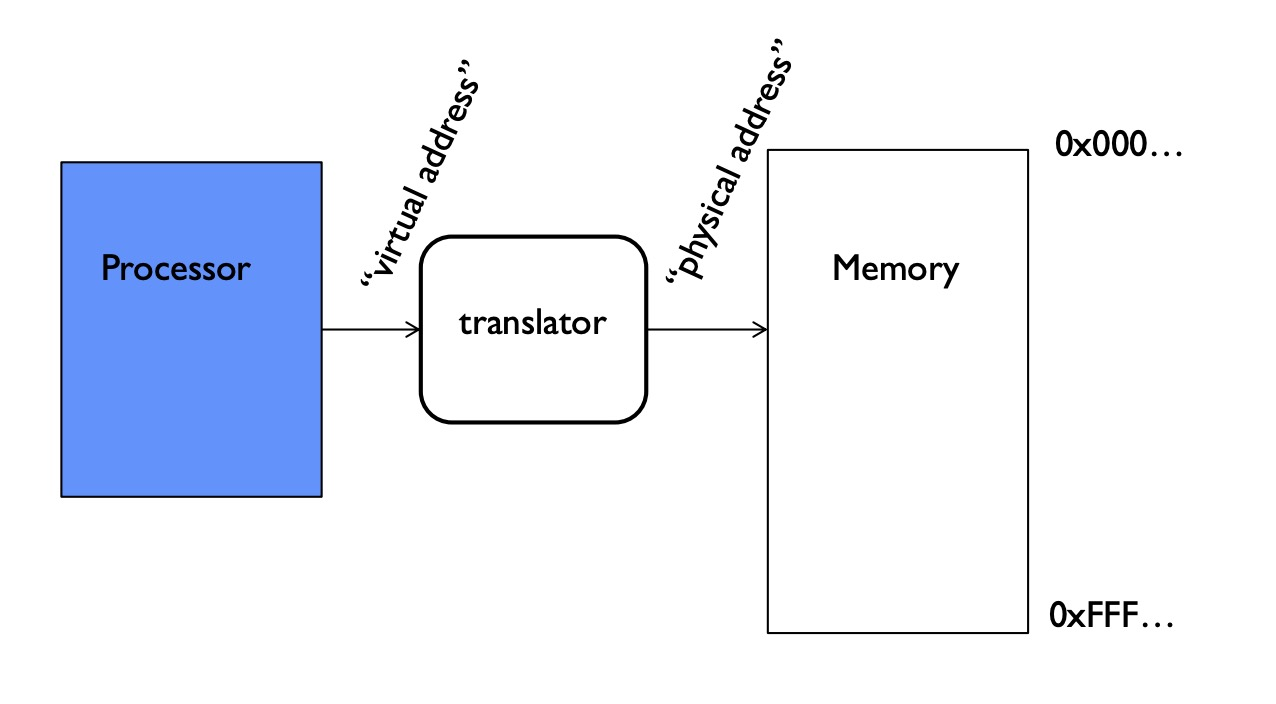
\includegraphics[width = 0.6\textwidth ]{figures/address_space_translation.jpg}
    \caption{Address Space Translation}
    % \label{fig:batteryIncreas}
\end{figure}

\begin{tcolorbox}
\begin{discussion}
How do we get the system target address of the
``unprogrammed control transfer?''
\end{discussion}    
\textbf{Interrupt Vector}
\end{tcolorbox}
\begin{example}
How does the context switch?
\end{example}

\begin{figure}[http]
\centering
\begin{minipage}[t]{0.48\textwidth}
    \centering
    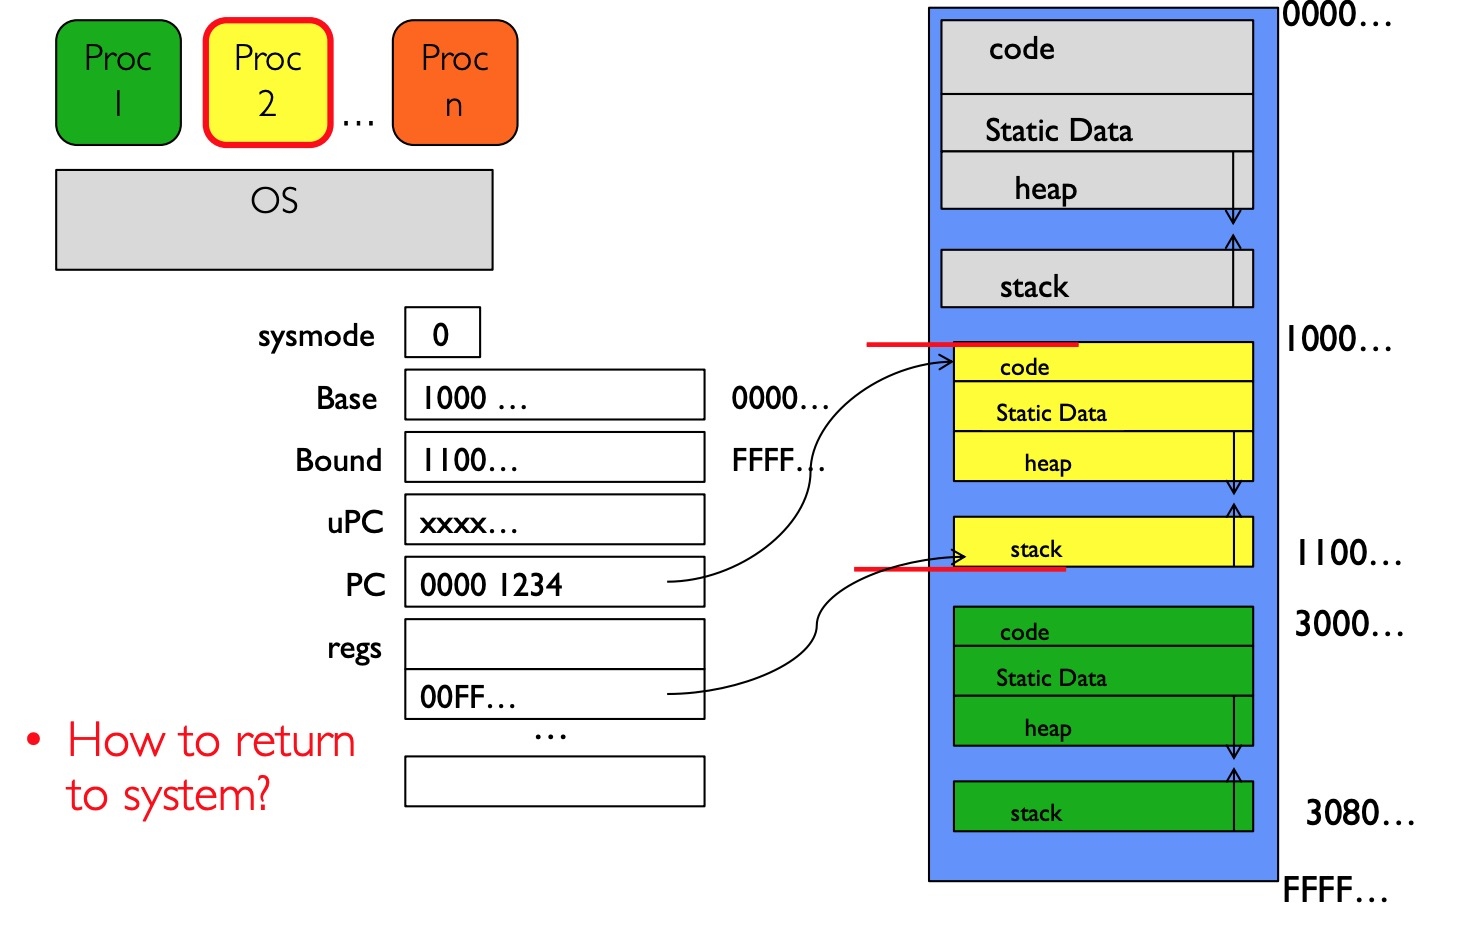
\includegraphics[width=7cm]{figures/from_user_to_kernel.jpg}
    \caption{From User to Kernel}
    % \label{fig:batteryIncreas}
    \end{minipage}
\begin{minipage}[t]{0.48\textwidth}
    \centering
    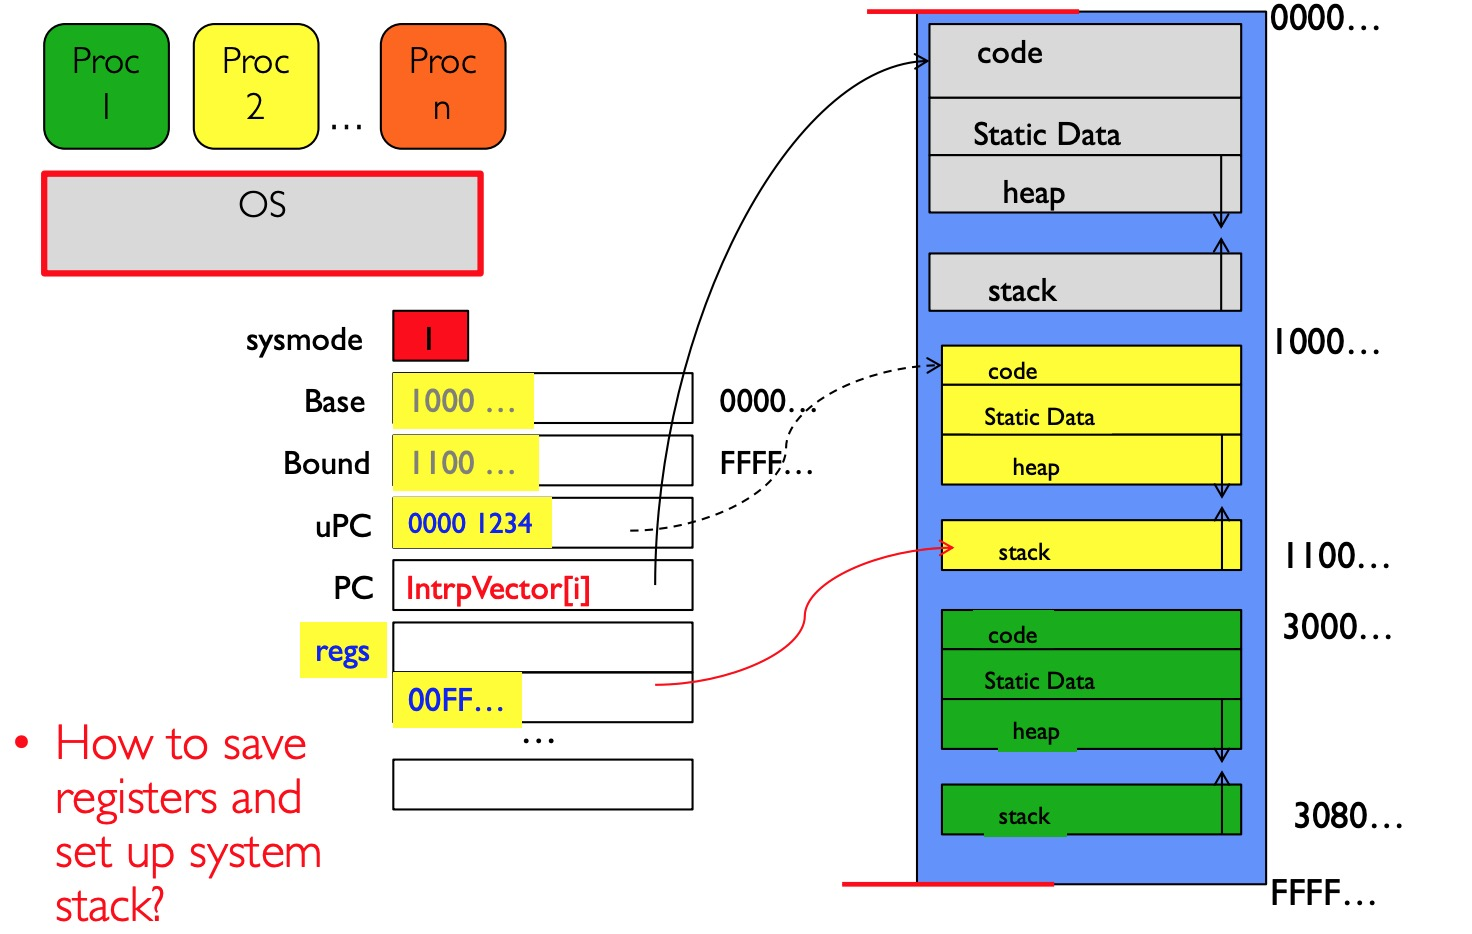
\includegraphics[width=7cm]{figures/interupt.jpg}
    \caption{Interrupt}
    % \label{fig:batteryIncreas}
    \end{minipage}
\end{figure}

\begin{figure}[http]
\centering
\begin{minipage}[t]{0.48\textwidth}
    \centering
    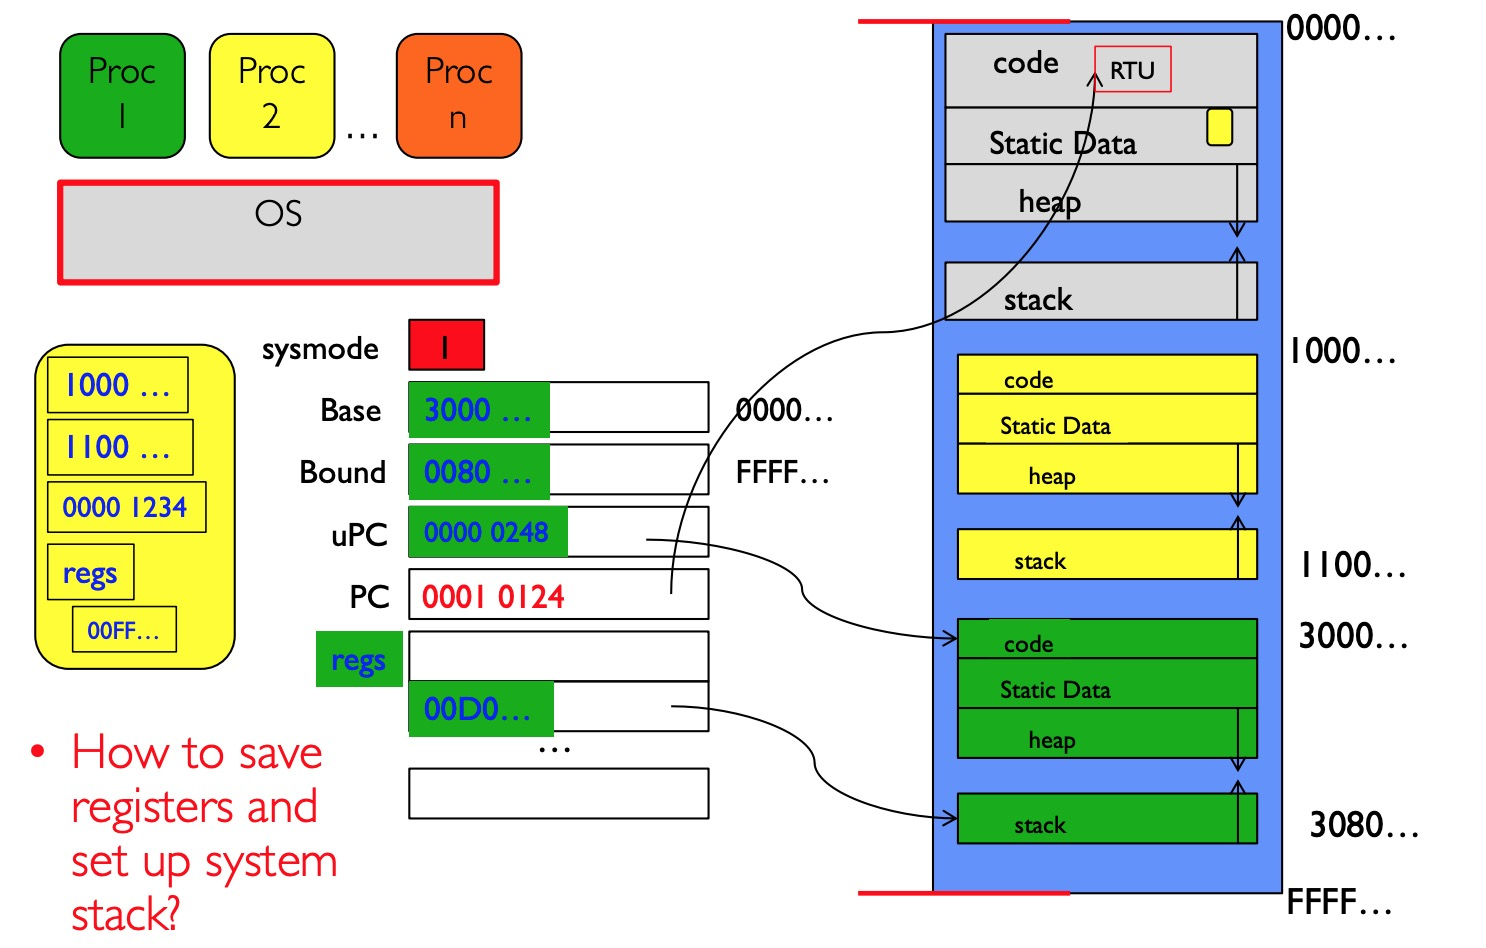
\includegraphics[width=7cm]{figures/switch.jpg}
    \caption{Switch User Process}
    % \label{fig:batteryIncreas}
    \end{minipage}
\begin{minipage}[t]{0.48\textwidth}
    \centering
    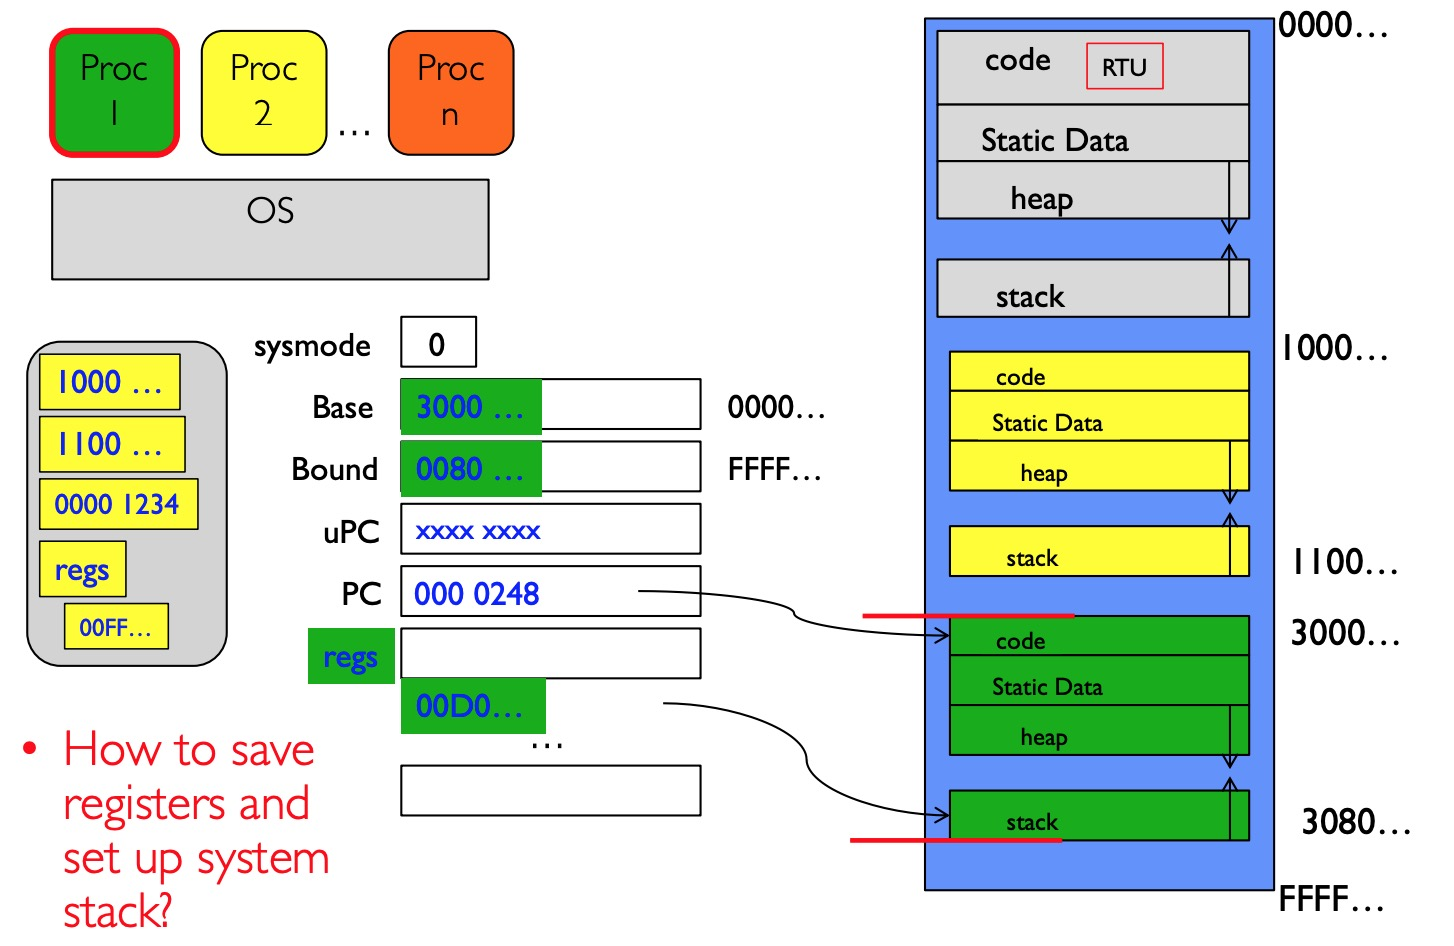
\includegraphics[width=7cm]{figures/resume.jpg}
    \caption{Resume}
    % \label{fig:batteryIncreas}
    \end{minipage}
\end{figure}
\subsubsection{Motivation for Threads}
Operating systems must handle multiple things at once (\textbf{MTAO})
\begin{itemize}
    \item Processes, interrupts, background system maintenance
\end{itemize}
Networked servers must handle \textbf{MTAO}
\begin{itemize}
    \item Multiple connections handled simultaneously
\end{itemize}
Parallel programs must handle \textbf{MTAO}
\begin{itemize}
    \item To achieve better performance
\end{itemize}
Programs with user interface often must handle \textbf{MTAO}
\begin{itemize}
    \item To achieve user responsiveness while doing computation
\end{itemize}
Network and disk bound programs must handle \textbf{MTAO}
\begin{itemize}
    \item To hide network/disk latency
    \item Sequence steps in access or communication
\end{itemize}

\begin{tcolorbox}
\begin{discussion}
Multiprocessing vs. Multiprogramming
\end{discussion}
\begin{itemize}
    \item \textbf{Multiprocessing}: Multiple CPUs (cores)
    \item \textbf{Multiprogramming}: Multiple jobs/processes
    \item \textbf{Multithreading}: Multiple threads/processes
\end{itemize}
\end{tcolorbox}

\subsubsection{Thread State}
State shared by all threads in process/address space
\begin{itemize}
    \item Content of memory (global variables, heap)
    \item I/O state (file descriptors, network connections, etc)
\end{itemize}

State “private” to each thread
\begin{itemize}
    \item Kept in \textbf{TCB} (Thread Control Block)
    \item CPU \textbf{registers} (including, program counter)
    \item Execution \textbf{stack}
\end{itemize}


\label{EndOfText}

\newpage
\pagenumbering{Roman} 
\addcontentsline{toc}{section}{List of Figures}
\fancyfoot[C]{Page \thepage\ of \pageref{endOfDoc}}
\listoffigures
\thispagestyle{fancy}

\newpage
\addcontentsline{toc}{section}{List of Tables}
\listoftables
\thispagestyle{fancy}

\newpage
\addcontentsline{toc}{section}{Nomenclature}
\makenomenclature
%\clearpage
%\mbox{}

\nomenclature{EV}{Electric Vehicle}
\nomenclature{AC}{Alternating Current}
\nomenclature{DC}{Direct Current}
\nomenclature{IGBT}{Insulated-gate Bipolar Transistor}
\nomenclature{PV}{Photovoltaics}
\nomenclature{RMS}{Root Mean Square}
\nomenclature{FCS}{Fast Charging Station}
\nomenclature{PMU}{Phase Measurement Unit}
\nomenclature{THD}{Total Harmonic Distortion}
\nomenclature{EMI}{Electromagnetic Interference}
\nomenclature{$h$}{Planck constant}
 
\printnomenclature

\newpage
\addcontentsline{toc}{section}{References}
\bibliography{document.bib} 
\bibliographystyle{ieeetr}

\newpage
\section{Appendix A} \label{ch6}

\label{endOfDoc}
\end{document}
